\label{instalacja_oprogramowania}Wraz z systemem Ubuntu na twoim dysku twardym znalazła się cała gama oprogramowania --- pakiet biurowy, przeglądarka internetowa, odtwarzacze multimediów, itd. Jednak zapewne chciałbyś zainstalować więcej programów, bardziej odpowiadających twoim potrzebom. W tym rozdziale przedstawione zostaną sposoby instalacji programów w systemie Ubuntu.

W systemach linuksowych (Ubuntu do nich należy) instalacja programów przebiega nieco inaczej, niż gdzie indziej, a jednocześnie bardzo podobnie. Jak to możliwe? Bardzo prosto. Zapewne znasz pojęcie ,,sklepu z oprogramowaniem''. Apple ma swój ,,App Store'', Google ma swoje ,,Play''. Są to stosunkowo nowe metody instalacji oprogramowania, które upowszechniły się w przeciągu ostatnich lat. Nawet Microsoft w najnowszych wydaniach swojego systemu Windows promuje instalację softu przez wbudowany sklep, zamiast ręcznego przeszukiwania sieci, ściągania instalatorów, skanowania ich antywirusem i instalowania w systemie.

Takie sklepy z oprogramowaniem istnieją w systemach linuksowych od dawna, przy czym w tym przypadku nazywają się \textcolor{ubuntu_orange}{repozytoriami}. Repozytorium to serwer, na którym opiekunowie danej dystrybucji Linuksa (np. firma Canonical jest opiekunem Ubuntu) przechowują paczki z programami. Użytkownik, chcąc coś zainstalować (np. przeglądarkę internetową Firefox), uruchamia program zwany \textcolor{ubuntu_orange}{menadżerem pakietów}, wyszukuje w nim to, czego potrzebuje i instaluje. Nic więcej go nie interesuje --- menadżer pakietów sam ściągnie paczkę z programem, pobierze wszystkie zależności (programy i~biblioteki niezbędne do funkcjonowania instalowanego programu) i zainstaluje soft w systemie. Kiedy w repozytoriach program zostanie zaktualizowany, użytkownik zostanie o tym powiadomiony, a~menadżer pakietów dokona aktualizacji.

W przeciwieństwie do sklepów z oprogramowaniem system repozytoriów przechowuje nie tylko programy użytkowe, ale też składniki systemu operacyjnego, sterowniki, dokumentację, pliki pomocy, paczki z tematami graficznymi i ikonami oraz wiele innych. Użytkownik nie jest też ograniczony wyłącznie do repozytoriów oferowanych przez opiekunów dystrybucji --- swobodnie może łączyć się z~innymi serwerami w celu poszerzenia oferty oprogramowania. W Ubuntu istnieje cały ekosystem repozytoriów PPA (\textit{Personal Package Archive}), które kilkoma kliknięciami można dodać do systemu. Deweloperzy różnych aplikacji za pośrednictwem PPA dostarczają użytkownikom oprogramowanie, które nie znalazło się w repozytoriach oferowanych przez Canonical.

Podstawową jednostką w repozytorium jest paczka. Jest to skompresowane archiwum, zawierające wszystkie pliki programu (czyli soft oraz dodatki: dokumentacja, ikony, grafiki, dźwięki i inne), a także informacje co i gdzie ma zostać wypakowane.

\subsubsection{Centrum Oprogramowania Ubuntu}
\textcolor{ubuntu_orange}{Centrum Oprogramowania Ubuntu} jest programem służącym do zarządzania zainstalowanymi aplikacjami. W przeciwieństwie do bardziej rozbudowanej klasy programów, zwanych menadżerami pakietów, Centrum Oprogramowania jest swego rodzaju sklepem z aplikacjami. Znajdziesz tu gotowe instalatory programów dostępnych w podstawowych repozytoriach, a także programy płatne. Z drugiej strony, nie ma tutaj pakietów z podstawowymi składnikami systemu.

\begin{center}
	\begin{tikzpicture}
	\node[anchor=south west,inner sep=0] (image) at (0,0) {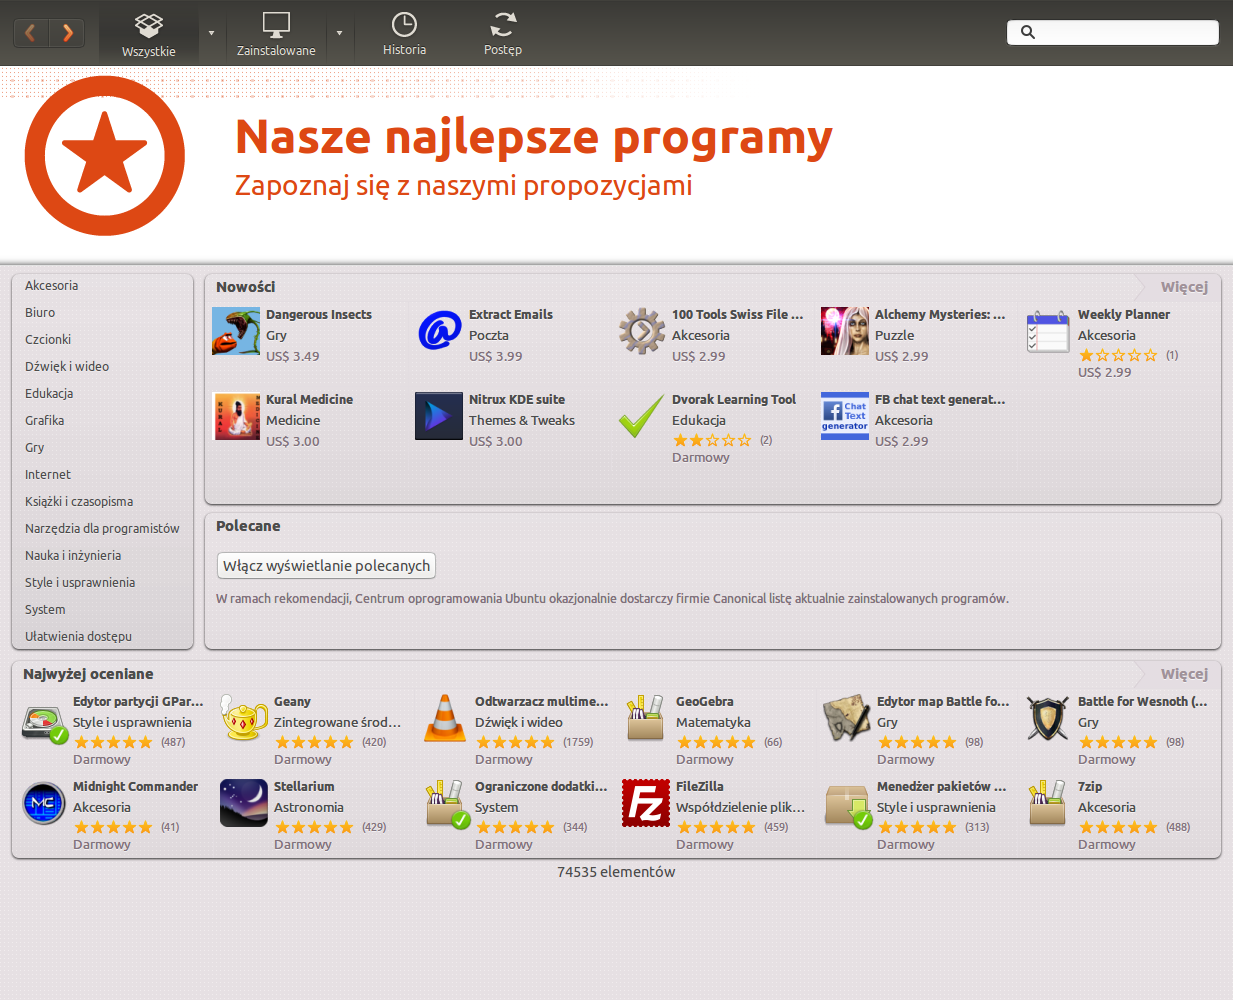
\includegraphics[width=\linewidth]{images/programy_centrum.png}};
	\begin{scope}[x={(image.south east)},y={(image.north west)}]
		\draw[ubuntu_orange,line width=3pt,rounded corners] (0.80,0.95) rectangle (0.99,0.99);
		\draw[ubuntu_orange,line width=3pt,fill=white,fill opacity=0.75] (0.65,0.97) circle [radius=0.30cm]
			node[text=black]{\Large \textbf 1};
		\draw[ubuntu_orange,dashed,line width=3pt] (0.67,0.97) -- (0.79,0.97);
		
		\draw[ubuntu_orange,line width=3pt,rounded corners] (0.01,0.35) rectangle (0.16,0.73);
		\draw[ubuntu_orange,line width=3pt,fill=white,fill opacity=0.75] (0.10,0.55) circle [radius=0.30cm]
			node[text=black]{\Large \textbf 2};
	\end{scope}
\end{tikzpicture}
\end{center}

W prawym górnym rogu znajduje się pole \circled 1, w którym można wpisać nazwę szukanego programu (lub jej część), a Centrum Oprogramowania Ubuntu wyświetli wyniki wyszukiwania. Środkowa część ekranu zawiera polecane i najwyżej oceniane aplikacje. Z lewej strony \circled 2 jest lista kategorii oprogramowania:
\begin{itemize}
\item \textcolor{ubuntu_orange}{Akcesoria}: niewielkie programy, pomocne w codziennym używaniu komputera;
\item \textcolor{ubuntu_orange}{Biuro}: programy biurowe, bardziej rozbudowane edytory tekstu, arkusze kalkulacyjne, organizery i inne;
\item \textcolor{ubuntu_orange}{Czcionki}: dodatkowe zestawy fontów;
\item \textcolor{ubuntu_orange}{Dźwięk i wideo}: zawiera oprogramowanie do tworzenia i odtwarzania multimediów;
\item \textcolor{ubuntu_orange}{Edukacja}: programy wspomagające nauczanie i różnego rodzaju bazy wiedzy;
\item \textcolor{ubuntu_orange}{Grafika}: programy do grafiki wektorowej i rastowej, a także przeglądarki grafiki, programy do wywoływania i korekcji zdjęć;
\item \textcolor{ubuntu_orange}{Gry}: oprogramowanie rozrywkowe;
\item \textcolor{ubuntu_orange}{Internet}: różnego rodzaju oprogramowanie do wymiany danych z internetem (przeglądarki internetowe, klienty poczty email, programy do transmisji danych, klienty Bittorrent);
\item \textcolor{ubuntu_orange}{Książki i czasopisma}: publikacje (najczęściej płatne) poświęcone Linuksowi i otwartemu oprogramowaniu;
\item \textcolor{ubuntu_orange}{Narzędzia dla programistów}: kompilatory, IDE, biblioteki programistyczne i dokumentacja;
\item \textcolor{ubuntu_orange}{Nauka i inżynieria}: programy dotyczące różnych dziedzin nauki (matematyki, chemii, fizyki, astronomii, itd), a także do komputerowego wspomagania projektowania (CAD);
\item \textcolor{ubuntu_orange}{Style i usprawienia}: zestawy ikon oraz stylów graficznych dla Ubuntu;
\item \textcolor{ubuntu_orange}{System}: narzędzia systemowe, różnego rodzaju konfiguratory;
\item \textcolor{ubuntu_orange}{Ułatwienia dostępu}: programy dla niepełnosprawnych.
\end{itemize}

\subsubsection{Menadżer pakietów Synaptic}
Bardziej rozbudowaną aplikacją do zarządzania paczkami z oprogramowaniem jest menadżer pakietów \textcolor{ubuntu_orange}{Synaptic}. Nie jest on standardowo instalowany w systemie, ale bez problemu można go znaleźć w Centrum Oprogramowania Ubuntu.

Synaptic wyświetla pełną listę pakietów aktualnie dostępnych w repozytoriach Ubuntu oraz wszystkich repozytoriach dodanych w trakcie używania systemu. W przeciwieństwie do Centrum Oprogramowania, Synaptic pokazuje nazwę pakietu z programem, a nie jego nazwę.

Aby zainstalować program z użyciem Synaptica, kliknij checkbox obok nazwy pakietu i z rozwiniętego menu wybierz \textcolor{ubuntu_orange}{Zaznacz do instalacji}. Synaptic sprawdzi jakie inne pakiety są niezbędne do działania danego programu i zaproponuje ich instalację. Możesz zaznaczyć wiele programów do instalacji za jednym zamachem. Zmiany są wprowadzane dopiero po kliknięciu \textcolor{ubuntu_orange}{Zastosuj} na górnej belce narzędziowej.

Synaptic, poza przeglądaniem i instalowaniem oprogramowania, umożliwia także reinstalację programu, aktualizację (tak samo jak aktualizacje systemowe), usunięcie oraz całkowite usunięcie (wraz z plikami konfiguracyjnymi i innymi pozostałościami) paczki z systemu.

\begin{center}
	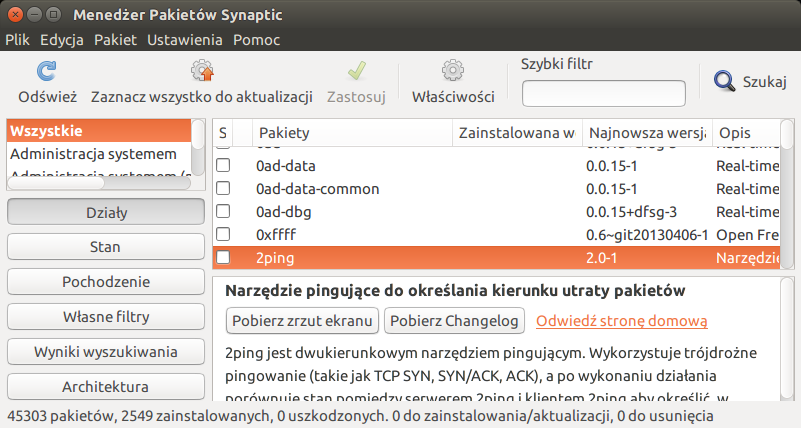
\includegraphics[width=\linewidth]{images/programy_synaptic.png}
\end{center}

\subsubsection{Instalacja programów w konsoli}
Graficzne narzędzia są wygodne, ale czasem trzeba sięgnąć po konsolę. Często na forach pomocy technicznej właśnie ten sposób jest przedstawiany w opisach metod rozwiązywania problemów. Łatwiej wpisać jedno polecenie w konsoli, niż opisywać, jak przedostać się przez gąszcz menu i przycisków. Wynika to z założenia, że nie każdy musi mieć zainstalowany menadżer pakietów. Nawet Centrum Oprogramowania może być nieobecne w systemie --- to program jak każdy inny i może zostać usunięty.
W dalszych częściach tego Przewodnika kilkukrotnie przedstawiamy instalację paczek właśnie w ten sposób.

Konsolowym menadżerem pakietów w systemie Ubuntu jest \textcolor{ubuntu_orange}{apt-get}. Ma on takie same możliwości jak opisywany wcześniej Synaptic, z tym, że polecenia wydaje się klawiaturą, a nie myszą. Aby zainstalować pakiet z oprogramowaniem przy pomocy apt-get:
\begin{enumerate}
\item Uruchom konsolę, wpisując w Dashu \textcolor{ubuntu_orange}{Terminal} lub wciskając kombinację klawiszy \keys{CTRL + Alt + t}.
\item Wpisz:
\begin{lstlisting}[language=bash]
sudo apt-get install vlc
\end{lstlisting}
\item Wciśnij \keys{\returnwin}
\item Wpisz swoje hasło i wciśnij \keys{\returnwin}. Nie przejmuj się, że hasło się nie pojawia. Jest to zabezpieczenie przed podglądaczami.
\end{enumerate}

VLC jest znanym na całym świecie kombajnem do odtwarzania wszelkiego rodzaju multimediów. Nie ma go w standardowej instalacji Ubuntu, ale dostępny jest za pośrednictwem repozytoriów. Co oznaczają poszczególne części tego polecenia?

\begin{itemize}
\item \textcolor{ubuntu_orange}{sudo} --- instalacja pakietów (a także ich usuwanie) wymaga uwierzytelnienia i tylko administrator systemu może to zrobić. \textit{Sudo} jest programem umożliwiającym wykonanie kolejnego polecenia przez innego użytkownika (w tym wypadku roota, administratora). Spróbuj wpisać to polecenie bez sudo na początku i zobacz, co się stanie.
\item \textcolor{ubuntu_orange}{apt-get} --- to konsolowy program do zarządzania pakietami.
\item \textcolor{ubuntu_orange}{install} --- \textit{install} to jedno z poleceń programu apt-get. W tym wypadku nakazuje mu zainstalować program.
\item \textcolor{ubuntu_orange}{vlc} --- nazwa programu, który chcesz zainstalować. Zwróć uwagę, że nazwy programów pisane są zawsze małymi literami, a także podawane są bez rozszerzenia.
\end{itemize}

Po podaniu hasła apt-get przetworzy żądanie (zainstaluj pakiet vlc) i wyświetli informację podobną do poniższej:

\begin{lstlisting}[language=bash]
Czytanie list pakietów... Gotowe
Budowanie drzewa zależności       
Odczyt informacji o stanie... Gotowe
Zostaną zainstalowane następujące dodatkowe pakiety:
  libbasicusageenvironment0 libcddb2 libcrystalhd3 libdvbpsi8 libebml4 libgnutls28 libgroupsock1
  libhogweed2 libiso9660-8 liblivemedia23 libmatroska6 libproxy-tools libresid-builder0c2a
  libsdl-image1.2 libsidplay2 libssh2-1 libtar0 libupnp6 libusageenvironment1 libva-x11-1
  libvcdinfo0 libvlc5 libvlccore7 libxcb-composite0 libxcb-keysyms1 libxcb-xv0 vlc-data vlc-nox
  vlc-plugin-notify vlc-plugin-pulse
Sugerowane pakiety:
  firmware-crystalhd gnutls-bin videolan-doc
Polecane pakiety:
  libdvdcss2
Zostaną zainstalowane następujące NOWE pakiety:
  libbasicusageenvironment0 libcddb2 libcrystalhd3 libdvbpsi8 libebml4 libgnutls28 libgroupsock1
  libhogweed2 libiso9660-8 liblivemedia23 libmatroska6 libproxy-tools libresid-builder0c2a
  libsdl-image1.2 libsidplay2 libssh2-1 libtar0 libupnp6 libusageenvironment1 libva-x11-1
  libvcdinfo0 libvlc5 libvlccore7 libxcb-composite0 libxcb-keysyms1 libxcb-xv0 vlc vlc-data
  vlc-nox vlc-plugin-notify vlc-plugin-pulse
0 aktualizowanych, 31 nowo instalowanych, 0 usuwanych i 0 nieaktualizowanych.
Konieczne pobranie 10,4 MB archiwów.
Po tej operacji zostanie dodatkowo użyte 51,3 MB miejsca na dysku.
Kontynuować? [T/n] 
\end{lstlisting}

To dużo tekstu, ale bardzo łatwo go zinterpretować:

\begin{itemize}
\item \textcolor{ubuntu_orange}{Czytanie list pakietów... Gotowe} --- apt-get przetworzył bazę danych pakietów i znalazł na liście program VLC.
\item \textcolor{ubuntu_orange}{Budowanie drzewa zależności} --- apt-get sprawdził jakich innych pakietów potrzebuje VLC do działania.
\item \textcolor{ubuntu_orange}{Zostaną zainstalowane następujące dodatkowe pakiety:} --- lista pakietów, które muszą być zainstalowane razem z programem VLC, aby mógł on działać.
\item \textcolor{ubuntu_orange}{Sugerowane pakiety:} --- lista przydatnych pakietów, które nie zostaną teraz zainstalowane, ale mogą się kiedyś przydać.
\item \textcolor{ubuntu_orange}{Polecane pakiety:} --- podobnie jak sugerowane pakiety, ale z większym naciskiem na przydatność. W tym wypadku apt-get zaproponował instalację biblioteki umożliwiającej odtwarzanie zaszyfrowanych płyt DVD. Ta paczka została omówiona w rozdziale \ref{ubuntu-restricted-extras}.
\item \textcolor{ubuntu_orange}{Zostaną zainstalowane następujące NOWE pakiety:} --- lista wszystkich pakietów, które zostaną zainstalowane. Automatyczna instalacja sugerowanych i polecanych pakietów domyślnie jest wyłączona.
\item \textcolor{ubuntu_orange}{0 aktualizowanych, 31 nowo instalowanych, 0 usuwanych i 0 nieaktualizowanych.} --- podsumowanie. Niektóre paczki są w konflikcie ze sobą (np. różne wersje tego samego programu) i instalacja jednej wymusza odinstalowanie innej.
\item \textcolor{ubuntu_orange}{Konieczne pobranie 10,4 MB archiwów.} --- ilość danych, jaka zostanie  pobrana z internetu.
\item \textcolor{ubuntu_orange}{Po tej operacji zostanie dodatkowo użyte 51,3 MB miejsca na dysku.} --- ilość miejsca, jaka zostanie zajęta po tej operacji.
\item \textcolor{ubuntu_orange}{Kontynuować? [T/n]} --- wciśnij \keys{t}, aby rozpocząć pobieranie i instalację, lub \keys{n}, aby przerwać procedurę.
\end{itemize}

Apt-get pobierze teraz wszystkie paczki, sprawdzi ich spójność (sumy kontrole oraz podpisy cyfrowe), rozpakuje je w systemie plików zgodnie z instrukcjami zawartymi w paczce i skonfiguruje zainstalowane programy (np. poinformuje menadżer plików, że teraz filmy ma odtwarzać w VLC, a~nie w domyślnie zainstalowanym Totemie).
\clearpage
Inne opcje programu apt-get to:

\begin{itemize}
\item \textcolor{ubuntu_orange}{update} --- pobiera z serwerów repozytoriów aktualną listę pakietów;
\item \textcolor{ubuntu_orange}{upgrade} --- aktualizuje wszystkie zainstalowane pakiety;
\item \textcolor{ubuntu_orange}{dist-upgrade} --- aktualizuje wszystkie zainstalowane pakiety, a także dokonuje instalacji nowych pakietów wskazanych przez aktualizacje (lub usuwa już niepotrzebne);
\item \textcolor{ubuntu_orange}{check} --- sprawdza stan zainstalowanych pakietów; wyświetli informację, jeżeli czegoś brakuje lub jakieś paczki są niepotrzebne;
\item \textcolor{ubuntu_orange}{remove} --- usuwa z systemu wskazaną paczkę;
\item \textcolor{ubuntu_orange}{purge} --- usuwa z systemu wskazaną paczkę wraz z pozostałościami (pliki konfiguracyjne, dokumentacja, logi itp.).
\end{itemize}

\subsubsection{Instalacja dodatkowych repozytoriów}
W standardowych repozytoriach Ubuntu znajduje się około 45 tysięcy paczek. Liczba ta wydaje się ogromna, ale jest to jedynie ułamek dostępnego oprogramowania. Te 45 tysięcy pakietów jest zarządzane i sprawdzane przez Canonical, lecz nie ma możliwości, aby dbał on o każdy inny, choćby najmniejszy program. Dlatego w ręce deweloperów aplikacji został oddany mechanizm PPA. Najczęściej zarejestrowanie takiego PPA w systemie opisywane jest jako szereg trzech komend, które trzeba wydać w terminalu. W tym przykładzie zarejestrujemy PPA zawierające pakiet biurowy LibreOffice (a ściślej aktualizacje tego zestawu programów, które nie trafiły na serwery Canonicalu).
\begin{enumerate}
\item Dodaj repozytorium:
\begin{lstlisting}[language=bash]
sudo apt-add-repository ppa:libreoffice/ppa
\end{lstlisting}
Przy każdym dodawanym PPA program wyświetli skrócone informacje. Zapoznaj się z nimi i wciśnij \keys{\returnwin}, aby dodać to repozytorium do systemu, lub \keys{ctrl + c}, aby przerwać operację.
\item Zaktualizuj listę pakietów:
\begin{lstlisting}[language=bash]
sudo apt-get update
\end{lstlisting}
\item Zainstaluj LibreOffice:
\begin{lstlisting}[language=bash]
sudo apt-get install libreoffice
\end{lstlisting}
\end{enumerate}

Aby dodać repozytorium w sposób graficzny, wykonaj następujące czynności:
\begin{enumerate}
\item Wyszukaj w Dashu, a następnie uruchom \textcolor{ubuntu_orange}{Oprogramowanie i aktualizacje}.
\item Przejdź do zakładki \textcolor{ubuntu_orange}{Inne oprogramowanie}.
\item Kliknij przycisk \textcolor{ubuntu_orange}{Dodaj}.
\item W pole \textcolor{ubuntu_orange}{Wiersz APT} wpisz adres repozytorium, tutaj: \textit{ppa:libreoffice/ppa}.
\item Kliknij \textcolor{ubuntu_orange}{Dodaj zasób}, a nastepnie \textcolor{ubuntu_orange}{Zamknij}.
\item Zostaniesz poproszony o zaktualizowanie listy pakietów. Wykonaj tę czynność.
\end{enumerate}

\subsubsection{Instalacja pakietów .deb}
Niektórzy twórcy programów nie opiekują się własnymi repozytoriami, ale zamiast tego przygotowują paczki z oprogramowaniem do ręcznej instalacji. Takie paczki mają rozszerzenie \textit{.deb}. Identyczne paczki są pobierane z repozytoriów za pomocą Centrum Oprogramowania, Synaptica albo apt-get, z tym, że proces rozwiązywania zależności jest przez te programy prowadzony automatycznie, zaś podczas ręcznej instalacji paczek .deb --- nie.

Aby zainstalować pobraną paczkę .deb, masz dwie możliwości. W konsoli:
\begin{lstlisting}[language=bash]
sudo dpkg -i nazwa_paczki.deb
\end{lstlisting}
\begin{itemize}
\item \textcolor{ubuntu_orange}{sudo} --- instalacja pakietów (a także ich usuwanie) wymaga uwierzytelnienia i tylko administrator systemu może to zrobić;
\item \textcolor{ubuntu_orange}{dpkg} --- to konsolowy program do zarządzania paczkami .deb;
\item \textcolor{ubuntu_orange}{-i} --- polecenie programu dpkg, nakazujące mu zainstalować wskazaną paczkę;
\item \textcolor{ubuntu_orange}{nazwa\_paczki.deb} --- nazwa (ewentualnie poprzedzona ścieżką dostępu) wcześniej pobranej paczki.
\end{itemize}

Po takiej operacji raczej na pewno otrzymasz komunikat o ,,niespełnionych zależnościach''. Dpkg nie pobierze i nie zainstaluje brakujących pakietów. Na szczęście apt-get potrafi to naprawić. Wykonaj:
\begin{lstlisting}[language=bash]
sudo apt-get install -f
\end{lstlisting}

Polecenie \textcolor{ubuntu_orange}{install} z opcją \textcolor{ubuntu_orange}{-f} informuje apt-get, że ma sprawdzić stan paczek oraz zreperować (,,f'', czyli \textit{fix}) stan pakietów. Po tej operacji program zostanie prawidłowo zainstalowany i skonfigurowany, a~paczkę .deb można skasować.

Aby graficznie zainstalować pobraną paczkę .deb, potrzebujesz odpowiedniego programu. Nazywa się on \textcolor{ubuntu_orange}{GDebi}. Znajdziesz go w Centrum Oprogramowania, Synapticu lub zainstalujesz z konsoli poleceniem:
\begin{lstlisting}[language=bash]
sudo apt-get install gdebi
\end{lstlisting}

Kiedy GDebi jest gotowe do użycia, kliknij prawym przyciskiem myszy paczkę .deb, a następnie wybierz \menu{{Otwórz za pomocą}>{GDebi Package Installer}}. Teraz wystarczy kliknąć \textcolor{ubuntu_orange}{Install}, aby GDebi sprawdziło zależności i zainstalowało wszystko, co potrzebne.

\subsubsection{Instalacja programów .bin}
Niektórzy dostawcy oprogramowania (na szczęście nieliczni) udostępniają własne instalatory programów, na sposób znany z systemu Windows (pliki .exe i .msi). Na szczęście są to coraz rzadsze przypadki. Jednak gdybyś przypadkiem trafił na tak przestarzały sposób dystrybucji programu, to kliknij prawym przyciskiem myszy na pobranym programie, wybierz \menu{{Właściwości}>{Uprawienia}>{Wykonywanie}} i~zaznacz pole \textcolor{ubuntu_orange}{Zezwolenie na wykonywanie pliku jako programu}. Teraz kliknij dwukrotnie lewym przyciskiem myszy na pliku, aby go uruchomić.

\subsubsection{Instalacja programów przez przeglądarkę internetową}
Przeglądarka internetowa Firefox, wchodząca w skład standardowej instalacji Ubuntu, wyposażona jest w dodatek umożliwiający instalację oprogramowania bezpośrednio ze strony internetowej poprzez protokół apt. Kliknięcie odpowiedniego linku otworzy okno \textcolor{ubuntu_orange}{Centrum Oprogramowania Ubuntu} na stronie danego programu.

Jeżeli Firefox nie rozpoznaje protokołu apt, to wyświetli okno z prośbą o wybór aplikacji. Kliknij przycisk \textcolor{ubuntu_orange}{Wybierz\ldots}, a następnie wskaż plik \menu{{System plików}>{usr}>{bin}>{software-center}}. Pamiętaj, aby zaznaczyć pole \textcolor{ubuntu_orange}{Zapamiętaj wybór dla odnośników apt}.
\clearpage
